%% The following is a directive for TeXShop to indicate the main file
%%!TEX root = diss.tex
\chapter{AtomicOpt.jl: a Julia package for structured optimiztaion}
\label{ch:App-AtomicOpt}

\section{Introduction} \label{sec:5-1}
In this chapter, we introduce a open-source Julia package \texttt{AtomicOpt.jl}\footnote{\url{https://github.com/MPF-Optimization-Laboratory/AtomicOpt.jl}} for solving a class of structured optimization problems. All the numerical experiments in \autoref{ch:Dual-Struc-Opt}, \autoref{ch:App-Sig-Demix} and \autoref{ch:App-Primal-Retrieval} are conducted using this package. 

\texttt{AtomicOpt.jl} aims to solve the following cardinality-constrained problem:
\begin{equation} \label{eq:main_prob_atomic_opt} 
\begin{split}
  \find & x_1, \dots, x_k \in \Re^n \\
  \sut  & \left\|M\left(\sum_{i=1}^k x_i\right) - b \right\| \leq \alpha \tand \\
        & \card\Asi(x_i) \leq r_i \enspace \forall i \in [k],
\end{split}
\end{equation}
where $m, n, k, r_i ~\forall i\in[k]$ are positive integers, $\alpha$ is a positive scalar indicating the constraint on the data-fitting term, $M: \Re^n \to \Re^m$ is a linear operator with $m < n$, $b \in \Re^m$ is the observation vector, $\Ascr_i \subseteq \Re^n$ is the basic atomic set for any $i\in[k]$ such that the set of exposed atoms $\Escr\Asi$ \eqref{eq:exposed-atoms} can be efficiently found, and $\card\As$ is the cardinality function as defined in \eqref{eq-card-fcn}. 

The signal demixing problem introduced in \autoref{ch:App-Sig-Demix} can be expressed in the format of problem \eqref{eq:main_prob_atomic_opt}, which can be viewed as a generalized version of the problem \eqref{eq:main_prob} introduced in \autoref{ch:App-Primal-Retrieval}. 

As we introduced in \autoref{ch:App-Sig-Demix}, in practice, we can solve the convex relaxation to the problem \eqref{eq:main_prob_atomic_opt}. More specifically, we know that under mild conditions, the following assumption holds. 
\begin{assumption} \label{ass:atomic_opt}
There exist positive scalars $\lambda_i, i\in[k]$, such that the minimizers $\{x_i^*\}_{i=1}^k$ to the following structured optimization problem
\begin{equation} \label{eq:main_prob_atomic_opt_cvx} 
  \begin{split}
      x_1^*, \dots, x_k^* &\in \argmin{x_1, \dots, x_k \in \Re^n} \max_{i=1,\dots,k} \enspace \frac{1}{\lambda_i}\gauge\Asi(x_i) \sut \sum_{i=1}^k x_i = x^* \text{where}\\
      x^* &\in \argmin{x\in\Re^n} \gauge\As(x) \sut \|Mx- b\| \leq \alpha \text{with} \\
      \Ascr &\coloneqq \sum_{i=1}^k \lambda_i\Ascr_i
  \end{split}
\end{equation}
are feasible to problem \eqref{eq:main_prob_atomic_opt}. 
\end{assumption}

As we introduced in \autoref{ch:App-Primal-Retrieval}, for better space complexity, we can instead solve the following dual formulation to the problem \eqref{eq:main_prob_atomic_opt_cvx}:
\begin{equation} \label{eq:main_prob_atomic_opt_dual} 
    \min_{r\in\Re^m}\enspace \gauge\MAs(b-r) \sut \|r\| \leq \alpha.
\end{equation}
Then near-feasible solutions to problem \eqref{eq:main_prob_atomic_opt} can obtained via \autoref{alg:primal_recover}. 

We describe the whole procedure and the candidate algorithms in \autoref{sec:5-2}. Then in \autoref{sec:5-3}, we introduce the basic atomic sets we include in this package. Finally, we show some examples using \texttt{AtomicOpt.jl}. 


\section{Algorithms} \label{sec:5-2}

In this section, we describe a procedure for obtaining near-feasible solutions to problem \eqref{eq:main_prob_atomic_opt}. The procedure first solves the dual formulation \eqref{eq:main_prob_atomic_opt_dual} using an algorithm requiring only the storage of several vectors of length $m$, which represents the size of the data $b$. The algorithm depends on the level-set method \cite{berg2011sparse,berg2008probing} and a generalized version of the dual conditional gradient method (\autoref{algo:dual-conditional-gradient}), which we describe in \autoref{sec:level} and \autoref{sec:dcg} respectively. As we show in \autoref{sec:primal_retrieval}, the solutions to the problem \eqref{eq:main_prob_atomic_opt} is subsequently obtained via an unconstrained linear least-squares problem that uses information implicit in the dual vector. \autoref{alg-level-set} summarizes the overall procedure. 

\begin{algorithm}[t]
  \DontPrintSemicolon
  \SetKwComment{tcp}{\tiny [}{]}
  \caption{Main procedure implemented in \texttt{AtomicOpt.jl}.\label{alg-level-set}}
  \smallskip
  \KwIn{noise level $\alpha>0$; accuracy $\epsilon>0$}
  $\tau^{0} \gets 0$
 
  \For(\tcp*[f]{\tiny level-set iterations}){\nllabel{alg-level-set-loop}$t\gets0,1,2,\ldots$}{
    $(r\t,\, p\t,\, \ell\t)\leftarrow\texttt{DCG}(\tau\t)$ \tcp*{\tiny solve~\eqref{eq:value-fn} approximately}\nllabel{alg-level-set-cg}
    \lIf(\tcp*[f]{\tiny test $\epsilon$-infeasibility}){$\|r\t\| \leq \alpha + \epsilon$}{break}
    $\tau\tp1 \gets \tau\t + \frac{\ell\t-\alpha^2/2}{\ip{p\t}{r\t}}$\nllabel{alg-level-set-update}
    \tcp*{\tiny Newton update}
  }
   $(x_1,\ldots,x_k) \gets \mbox{solve~\eqref{eq:primal-recovery}}$ \nllabel{alg-primal-recovery}
   \tcp*{\tiny primal retrieval}
  \Return{$(x_1,\ldots,x_k)$}
 \end{algorithm}


\subsection{Level-set method} \label{sec:level}
The loop beginning at \autoref{alg-level-set-loop}  of \autoref{alg-level-set} describes the level-set method \cite{BergFriedlander:2008,berg2011sparse,aravkin2016levelset} for solving problem \eqref{eq:main_prob_atomic_opt_dual}. More specifically, it approximately solves a sequence of problems
\begin{equation} \label{eq:value-fn}
  v(\tau) \coloneqq \min_{r}\left\{\frac{1}{2}\|r\|^2 ~\big\vert~ \gauge\MAs(b-r) \leq \tau\right\}. 
\end{equation} 
parameterized by the scalar $\tau$ that defines the level-set constraint, which is also known as the value function. The level-set method constructs a monotonically-increasing sequence $\{\tau\t\}$ that converges to the leftmost root $\tau^*$ of the equation $v(\tau) = \half\alpha^2$,
which represents the fidelity constraint of problem~\eqref{eq:main_prob_atomic_opt_dual}. Under modest assumptions satisfied by this problem, the sequence $\tau\t\to\tau^*=\opt$, the optimal value of~\eqref{eq:main_prob_atomic_opt_dual}. Let $r_{\tau}$ denote the minimizer for $v(\tau)$, then for any $\tau \leq \tau^*$ satisfying $v(\tau) \leq (\alpha+\epsilon)^2/2$, $r_\tau$ is a super-optimal and $\epsilon$-feasible solution to~\eqref{eq:main_prob_atomic_opt_dual}, i.e., a solution $r$ satisfies 
\begin{equation} \label{eq:super-optimal}
  \gauge\MAs(b-r) \leq \opt \text{and} \|r\| \leq \alpha + \epsilon,
\end{equation}
where $\epsilon$ is a specified optimality tolerance. 

The level-set algorithm requires $\BigOh(\log(1/\epsilon))$ approximate evaluations of the optimization problem~\eqref{eq:value-fn} to achieve this optimality condition. Each approximate evaluation provides a global lower-minorant of $v$ that is used by a Newton-like update to the level-set parameter $\tau\t$; see line~\ref{alg-level-set-update}. An illustration of the idea of the level-set method is shown in~\autoref{fig:value_fn}. 

\begin{figure}[t] 
    \begin{subfigure}{.48\textwidth}
      \centering
      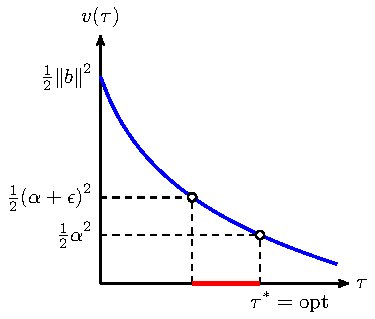
\includegraphics[width=\linewidth, page=1]{./figures/illustrations3}
      \captionsetup{justification=centering}
      \caption{Value function.}
    \end{subfigure}
    \hfill
    \begin{subfigure}{.48\textwidth}
      \centering
      \includegraphics[width=\linewidth, page=2]{./figures/illustrations3}
      \captionsetup{justification=centering}
      \caption{Newton-like update.}
    \end{subfigure}
    \captionsetup{justification=centering}
    \caption{Illustration of the level-set method.}
    \label{fig:value_fn}
\end{figure}

\subsection{Dual conditional gradient method} \label{sec:dcg}

\begin{algorithm}[t]
  \DontPrintSemicolon
  \setcounter{AlgoLine}{0}
  \SetKwComment{tcp}{\tiny [}{\tiny ]}
  \caption{Generalized dual conditional gradient method: \texttt{DCG}($\tau$). \label{alg:dcg}}
  \KwIn{$\tau$}

  $r^{(0)} \gets b$;\ $q_i^{(0)} \gets 0$ for all $i\in[k]$\;

  \For{$t\gets0,1,2,\ldots$}{
     $p_i\t \in \tau\lambda_i\Escr(M\Ascr_i;\,r\t)$ for all $i\in[k]$\tcp*{\tiny expose atoms}\nllabel{algo-expose-atom}
     $\Delta r_i\t\gets p_i\t-q_i\t$ for all $i\in[k]$\tcp*{\tiny compute $\Delta r$}
     $\rho\t \gets \ip{r\t}{\sum_{i=1}^k\Delta r_i\t}$\tcp*{\tiny optimality gap}
     \lIf(\tcp*[f]{\tiny break if optimal}){$\rho\t<\epsilon$}{
       break
     }
     $(\theta_1\t, \dots, \theta_k\t) \gets \mbox{solve~\eqref{eq:line_search}}$\tcp*{\tiny exact linesearch}\nllabel{algo-line-search}
     $r\tp1 \gets r\t - \sum_{i=1}^k \theta_i\Delta r_i\t$\tcp*{\tiny update $r$}
     $q_i\tp1 \gets q_i\t+\theta_i\t\Delta r_i\t$ for all $i\in[k]$\tcp*{\tiny update $q$}
  }
  $\ell\t\gets\half\|r\t\|^2-\rho\t$\tcp*{\tiny lower bound on optimal value}

  \Return{$r\t$, $\sum_{i=1}^k p_i\t$, $\ell\t$}
\end{algorithm}

The level-set subproblems are solved approximately using the generalized dual conditional-gradient method described by \autoref{alg:dcg}, which is generalized version of \autoref{algo:dual-conditional-gradient}. The main computational cost are in \autoref{algo-expose-atom} and \autoref{algo-line-search}. 

In \autoref{algo-expose-atom}, we use $r\t$ to expose atoms from $M\Ascr_i$, which can be implemented in parallel using the following identity, i.e.,
\begin{equation*}
  \Escr(M\Ascr_i;\,r\t) \equiv M\cdot\Escr(\Ascr_i, M^*r\t).
\end{equation*}
Recall that $\Ascr_i$ is the basic atomic set, so $\Escr(\Ascr_i, M^*r\t)$ can be efficiently computed. This formulation is convenient in cases where the operator $M$ can be applied implicitly to elements of the atomic set $\Ascr_i$. 

\autoref{algo-line-search} exhibits the exact linesearch, i.e., it solves the following box-constrained optimization problem
\begin{equation} \label{eq:line_search}
  \min_{\theta_1, \dots, \theta_k \in [0,1]} \enspace \left\|r\t - \sum_{i=1}^k \theta_i\Delta r_i\t\right\|.
\end{equation}
The exact linesearch problem \eqref{eq:line_search} is solved by using \texttt{LBFGSB.jl}\footnote{\url{https://github.com/Gnimuc/LBFGSB.jl}}, which is a Julia wrapper for the L-BFGSB-B algorithm developed by~\citet{zhu1997algorithm}. 

The conditional-gradient method converges to the required optimality within $\BigOh(1/\epsilon)$ iterations \cite{jaggi2013revisiting}. Combined with the complexity of the level-set method, we thus expect a total worst-case complexity of $\BigOh(\log(1/\epsilon)/\epsilon)$ iterations to satisfy the optimality condition~\eqref{eq:super-optimal}.

\subsection{Primal retrieval} \label{sec:primal_retrieval}
Once \autoref{alg-level-set} reaches \autoref{alg-primal-recovery}, the vector $r\t$ contains information about the atoms that are in the support of each of minimizers $x_i^*$ to the problem \eqref{eq:main_prob_atomic_opt_cvx}; cf. \autoref{th:polar-alignment}. According the result developed in \autoref{ch:App-Primal-Retrieval}, we can then obtain near-feasible solutions to the original cardinality-constrained problem \eqref{eq:main_prob_atomic_opt} via solving the following constrained optimization problem
\begin{equation} \label{eq:primal-recovery}
  \min_{x_1, \dots, x_k \in \Re^n} \enspace \left\|b - M\sum_{i=1}^k x_i\right\| \st x_i \in \texttt{EssCone}_{\Ascr_i, M, k_i}(r\t),
\end{equation}
where $\texttt{EssCone}$ is defined as in \eqref{eq:ess_cone}. The primal-retrieval problem \eqref{eq:primal-recovery} is solved by using \texttt{IterativeSolvers.jl}\footnote{\url{https://github.com/JuliaLinearAlgebra/IterativeSolvers.jl}}, which provides a Julia wrapper for the well-known conjugate gradient method.  



\section{Basic atomic sets} \label{sec:5-3}

In this section, we introduce some basic atomic sets implemented in \texttt{AtomicOpt.jl}. 

\paragraph{\texttt{OneBall}} refers to the atomic set described in \autoref{example-one-norm}. The basic usage is shown in the following code block. 
\begin{code}
  using AtomicOpt
  using LinearAlgebra
  using Test
  # set dimension
  n = 10
  # construct atomic set 
  A = OneBall(n)
  # generate random vector
  z = randn(n)
  # expose atom
  a = expose(A, z)
  # test
  @test dot(a,z) ≈ support(A, z)
\end{code}

\paragraph{\texttt{NucBall}} refers to the atomic set described in \autoref{example-nuclear-norm}. The basic usage is shown in the following code block. 
\begin{code}
  using AtomicOpt
  using LinearAlgebra
  using Test
  # set dimension
  n1, n2 = 10, 15
  # construct atomic set 
  A = NucBall(n1, n2)
  # generate random matrix
  z = randn(n1, n2)
  # expose atom
  a = expose(A, z)
  # test
  @test dot(a,z) ≈ support(A, z)
\end{code}

\paragraph{\texttt{TraceBall}} refers to the atomic set described in \autoref{example-trace-norm}. The basic usage is shown in the following code block. 
\begin{code}
  using AtomicOpt
  using LinearAlgebra
  using Test
  # set dimension
  n = 10
  # construct atomic set 
  A = TraceBall(n)
  # generate random matrix
  z = randn(n, n)
  # expose atom
  a = expose(A, z)
  # test
  @test dot(a,z) ≈ support(A, z)
\end{code}

\paragraph{\texttt{BlkNucBall}} refers to the atomic set described in \autoref{sec:3-5-4}. The basic usage is shown in the following code block. 
\begin{code}
  using AtomicOpt
  using LinearAlgebra
  using Test
  # set dimension
  n, bn = 10, 2
  # construct atomic set 
  A = BlkNucBall(n, n, bn, bn)
  # generate random matrix
  z = randn(n, n)
  # expose atom
  a = expose(A, z)
  # test
  @test dot(a,z) ≈ support(A, z)
\end{code}


\section{Examples} \label{sec:5-4}

In this section, we show how to use \texttt{AtomicOpt.jl} to solve some structured optimization problems introduced in \autoref{ch:Dual-Struc-Opt}, \autoref{ch:App-Sig-Demix} and \autoref{ch:App-Primal-Retrieval}. For simplicity, for the examples here we will use synthetic data. More examples with real data can be found on the GitHub page. 

\paragraph{Basis pursuit denoise} refers to the problem introduced in \autoref{ex:bpdn}. The following code block summarizes how to solve this problem using \texttt{AtomicOpt.jl}.
\begin{code}
  using AtomicOpt
  using LinearAlgebra
  using Printf
  import Random: seed!, randperm
  # set dimensions
  m, n, k = 2^8, 2^10, 8
  # random measurement operator
  M = randn(m, n) 
  # ground-truth signal with nnz = k
  p = randperm(n); p = p[1:k]; 
  x0 = zeros(n); x0[p] = randn(k)
  # noise
  η = randn(m)/100
  # measurement
  b = M*x0 + η
  # atomic set
  A = OneBall(n; maxrank=k)
  # solve the basis pursuit denoise problem
  sol = level_set(M, b, A, α = norm(η))
  # construct primal solution
  x = constructPrimal(sol)
  # report error
  @printf("relative difference between x0 and x: .2%f", norm(x - x0)/norm(x0))
\end{code}

\paragraph{Low-rank matrix completion} refers to the problem introduced in \autoref{ex:mc}. The following code block summarizes how to solve this problem using \texttt{AtomicOpt.jl}.
\begin{code}
  using AtomicOpt
  using LinearAlgebra
  using SparseArrays
  using Printf
  import Random: seed!, randperm
  # generate a random m×n matrix with rank r
  m, n, r = 100, 100, 3 
  X = rand(m, n)
  U, S, V = svd(X)
  X0 = U[:,1:r] * Diagonal( S[1:r] ) * V[:,1:r]'
  # generate a random mask with nnz ≈ m*n*p
  p = 0.5
  mask = sprand(Bool, m, n, p); 
  mask = convert(SparseMatrixCSC{Float64, Int64}, mask)
  # measurement
  B =  mask .* X0
  b =  B.nzval
  # operator
  Mop = MaskOP(mask)
  # atomic set
  A = NucBall(m, n, r)
  # solve the matrix completion problem
  sol = level_set(M, b, A, α = 0.0)
  # construct primal variable
  x = constructPrimal(sol)
  X = reshape(x, m, n)
  # Report recovery error
  @printf("relative difference between X0 and X: .2%f", norm(X - X0)/norm(X0))
\end{code}

\paragraph{Sparse and low rank matrix decomposition} refers to the problem introduced in \autoref{sec:3-5-3}. The following code block summarizes how to solve this problem using \texttt{AtomicOpt.jl}.
\begin{code}
  using AtomicOpt
  using LinearAlgebra
  using SparseArrays
  using Printf
  import Random: seed!, randperm
  # generate a random m×n matrix with rank r
  m, n, r = 100, 100, 3 
  X = rand(m, n)
  U, S, V = svd(X)
  x1 = U[:,1:r] * Diagonal( S[1:r] ) * V[:,1:r]'
  # generate a random m*n matrix with nnz ≈ m*n*p
  p = 0.01
  x2 = randn(m, n) .* sprand(Bool, m, n, p)
  k = nnz(x2)
  # measurement
  b = vec(x1 + x2)
  # atomic set
  A1 = NucBall(m, n, maxrank=r); A1 *= gauge(A1, xl)
  A2 = OneBall(m*n, maxrank=k); A2 *= gauge(A2, xs)
  A = A1 + A2
  # solve the sparse and low-rank decomposition problem
  sol = level_set(I(m*n), b, A, α = 0.0)
  # construct primal variable
  x = constructPrimal(sol)
  # Report recovery error
  @printf("relative difference for x1: .2%f", norm(x1 - x[1])/norm(x1))
  @printf("relative difference for x2: .2%f", norm(x2 - x[2])/norm(x2))
\end{code}


\section{Summary of contributions} \label{sec:5-5} 
In this chapter, we introduce our Julia package \texttt{AtomicOpt.jl} for solving structured optimization problems. The key design of this package depends on the level-set method, dual conditional gradient method and the primal-retrieval strategy developed in \autoref{ch:App-Primal-Retrieval}. All the numerical experiments conducted in \autoref{ch:Dual-Struc-Opt}, \autoref{ch:App-Sig-Demix} and \autoref{ch:App-Primal-Retrieval} are reproducible using \texttt{AtomicOpt.jl}. Note that \texttt{AtomicOpt.jl} provides not only a solver but also a framework for structured optimization. Users can easily add new basic atomic sets to it, as long as the implementation of the expose operation is known. 









